\chapter{Calculation of the boundaries at the target PS}\label{app:boundariescup}
\section{Analytical method to find the boundaries of the different regions in phase space}
In this section, we present an analytical method to find the boundaries of the regions formed by rays that follow the same path. Furthermore, we will represent those regions on source and target phase space.
%In the following we assume that the target is located immediately at the top of the cup.

%A path is defined as the collection of segments that constitute the ray when it propagates through the optical system.
%We will indicate with$.
It is possible to determine the maximum number of times that a ray reflects into the two-faceted cup as follows. Rotating the entire cup we can think of the path as a straight line that hits one of the rotated targets. The idea to rotate the cup comes from the fact that in this way we consider the paths as straight lines, hence it is sufficient to find only one intersection point between the ray and one line segment (also in the case where we have more than one reflection) and finally rotate back the intersection point to find the point on the target.
Next we want to explain this procedure in more detail.
Our optical system is defined as in the previous section, see Figure $\ref{fig:cup}$.
Let $B$ be defined by:
\begin{equation}\label{rotation}\begin{tabular}{llll}
$ B$ & $=$ & $ \big(h+\frac{a}{\tan(\gamma)}\big)\frac{1}{\cos(\gamma)}-\frac{a}{\tan(\gamma)}$ \\ $ \quad$ & $ \quad $ & $ \quad $ \\$ \quad$ &  $=$ & $\frac{h}{\cos(\gamma)}+a\tan\big(\frac{1}{2}\gamma\big),$\end{tabular}
\end{equation} and $P:(0,B)$ is the rotation point. We define $B_k$ as the clockwise ($k<0$) or counterclockwise ($k\geq 0$) rotations of the point $P:(0,B)$ over an angle $\alpha_k=(2k+1)\gamma$, with $\gamma$ the angle that the normal to the source forms with the reflectors of the cup and $ k\in \mathbb{Z} $ . The $x$ and $z$-coordinates of $B_k$ are indicated with $b_{k,x}$ and $b_{k,z}$, respectively, Figure $\ref{fig:twofaced}$ is illustrative.
\begin{figure}[htbp]%\label{fig:twofaced}
 \begin{center}
  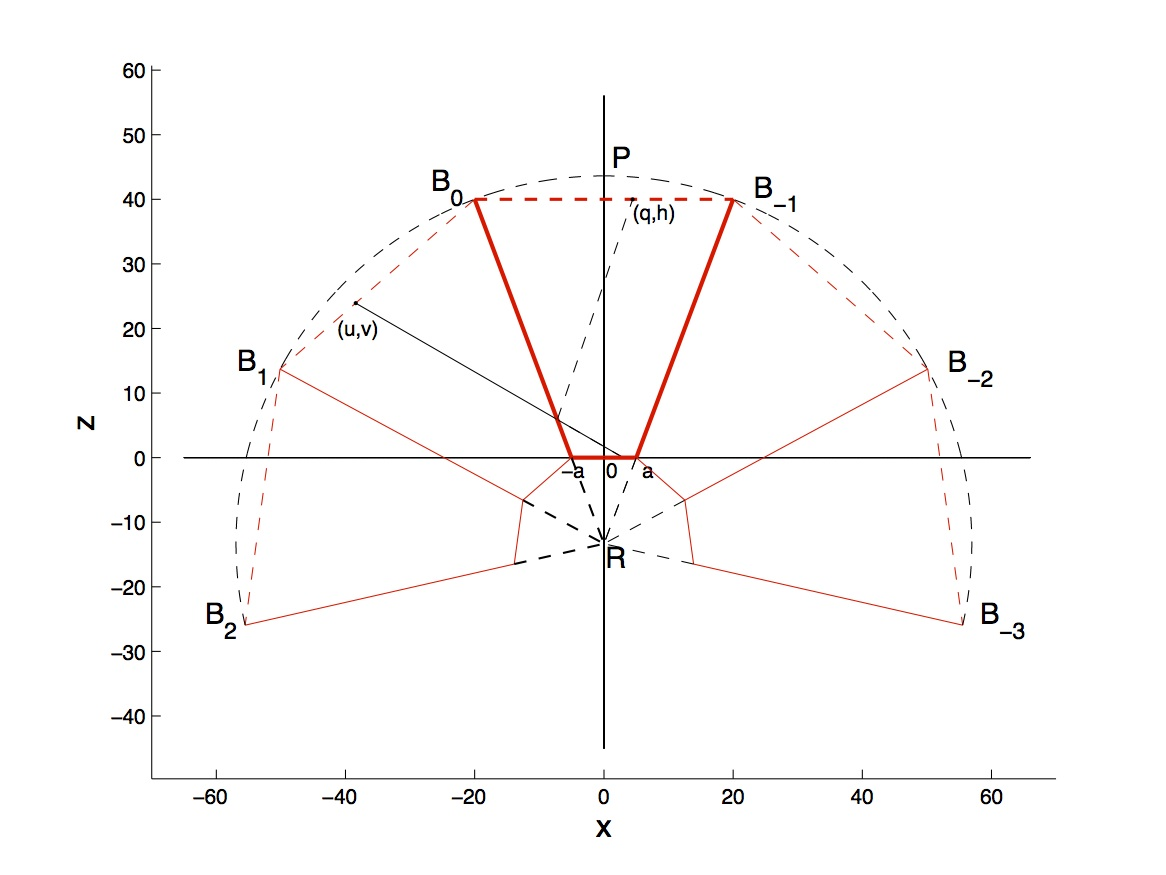
\includegraphics[width=10cm]{rotatedcup.jpg}
  \end{center}
 \caption{\footnotesize{The two-faceted cup rotated to both sides. The line segment $B_{k-1}B_{k}$ is the $|k|$ times rotated target. The point $(u,v)$ of the intersection between a ray and the segment $B_0B_1$ corresponds to the point $(q,h)$ on the target $B_{-1}B_{0}$. $P(0,B)$ is the point to rotate around the point $R = \big(0,-\frac{a}{\tan{\gamma}}\big)$. The length of the segments $RB_k$ is equal to the radius of the dashed circle.}}
  \label{fig:twofaced}
  \end{figure}
  %as the notation used in equation ($\ref{Bk}$) could suggest.
The position vector for the points $B_k$ is given by
$ \textbf{b}_k =
 \begin{pmatrix}   b_{k,x}\\  b_{k,z}
 \end{pmatrix} $
%\label{Bk}
where
\begin{equation}
 \textbf{b}_k+
  \begin{pmatrix} 0  \\  \frac{a}{\tan(\gamma)}\end{pmatrix}=
 \left(\begin{split}  & \cos(\alpha_k)  & -\sin(\alpha_k) \\  & \sin(\alpha_k) & \cos(\alpha_k)\end{split}\right)
 \begin{pmatrix}  0 \\  B+\frac{a}{\tan(\gamma)}\end{pmatrix}.
\end{equation}
Then the maximum number of reflections $r$ is:
\begin{equation}
r=\max\{k\in\mathbb{N} \;| \; b_{k-1,z}\geq 0\}\,.
\end{equation}
This method of rotating the cup instead of reflecting the ray inside the system can also be applied to find the boundaries of the regions
$M_{\textrm{s},k}$ and $M_{\textrm{t},k}$. In the following sections we will illustrate how this is done.
\\




\subsection{Source phase space}
We observe that the set of rays that form the boundary of the regions $M_{\textrm{s},k}$ only consists of rays that either leave the extremes of the source or hit one of the points
$B_k$. In Figure $\ref{fig:twofaced}$ is shown a ray that on the target phase space is located inside the region
$M_{\textrm{t},1}$, it does not constitute a point on any boundary. Furthermore, we note that the rays emitted from the corner points of the source form vertical lines in
$\mathcal{P}_\textrm{s}$, since $x = const$. On the other hand, rays that hit $B_k$ form vertical lines in $\mathcal{P}_\textrm{t}$, since $q = const$.
Hence for the representation on the source phase space we have to choose rays that hit $ B_{k} $, their directions are given by the relation \begin{equation}\label{anglesource}
\tan t = \frac{x-b_{k,x}}{b_{k,z}}\,.
\end{equation}
This is exactly what we did in the algorithm named \textit{'Source'} (see Appendix \ref{sec:source} for details).
\begin{figure}
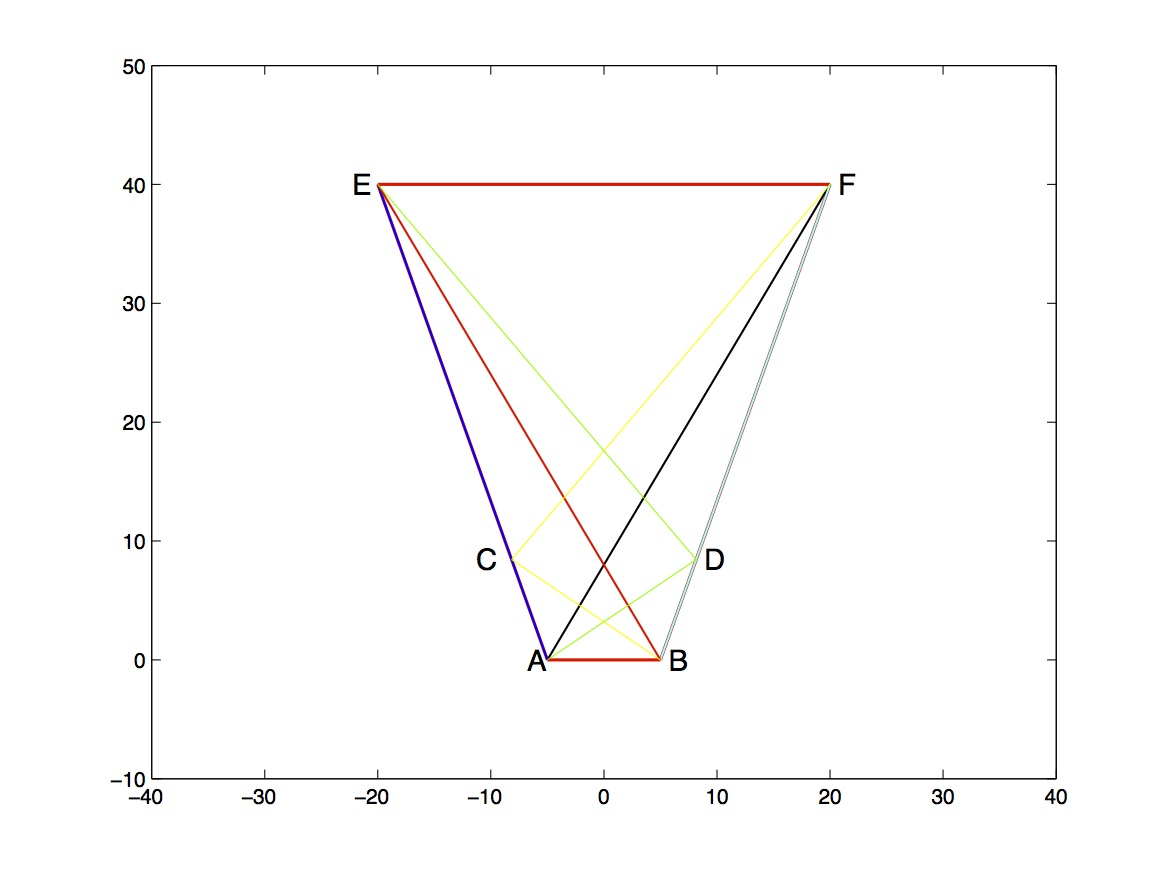
\includegraphics[scale=0.55]{raggi6.jpg}
\caption{\footnotesize{Rays that leave the corner points of the source. The rays $AF$, $BE$, $ACE$, $BDF$ are rays that do not hit the reflectors of the system.
They constitute rays on the boundaries of the regions $M_{\textrm{s},0}$, $M_{\textrm{s},1}$ and $M_{\textrm{s},-1}$.
 The rays $ADE$ and $BCF$ are rays that hit once the reflectors of the system. They constitute rays on the boundaries of the regions
 $M_{\textrm{s},-1}$, $M_{\textrm{s},-2}$, and $M_{\textrm{s},1}$ or $M_{\textrm{s},2}$, respectively.}}
\label{fig:raggi}
%\end{minipage}
\end{figure}

\begin{figure}[htbp]
%\centering
%\begin{minipage}[t]{.40\textwidth}
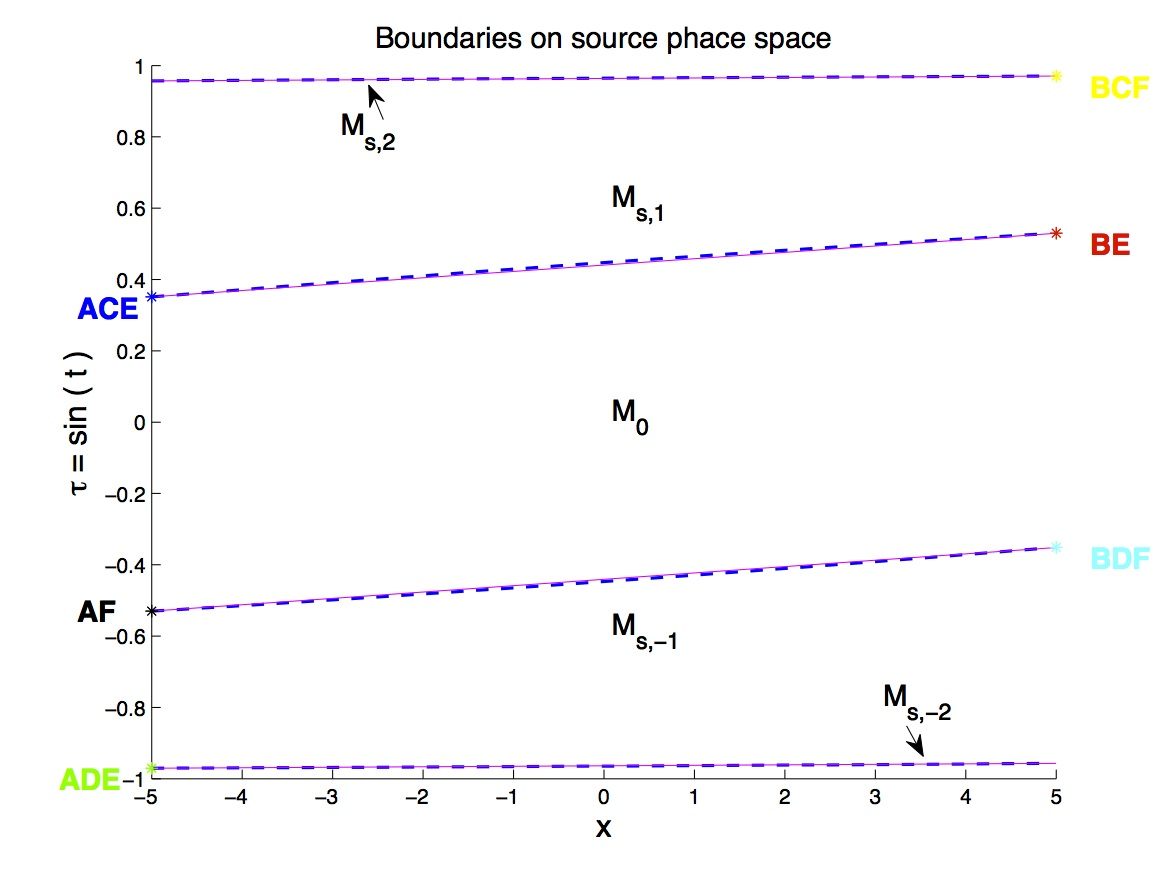
\includegraphics[scale=0.55]{boundaries_source.jpg}
\caption{\footnotesize{Regions $M_{s,k}$ of rays that reflect $|k|$ times, with $(x,\tau)\in\mathcal{P}_\textrm{s}$.
The parameter values are: $a=5$, $b=20$ and $h=40$. The continuous lines are the boundaries of the regions $M_{\textrm{s}}$
calculated considering rays that leave the source and hit the points $B_{k}$ at the target. The dashed blue lines are the boundaries calculated using ($\ref{anglesource}$) }}
\label{fig:boundary}
%\end{minipage} \qquad \qquad
%\begin{minipage}[t]{.40\textwidth}
\end{figure}
In Figure $\ref{fig:raggi}$ are shown some rays that compose the boundaries of $M_{\textrm{s},k}$ which coordinates are:
$$ \begin{array}{cc}ADE = \Bigg(-a, \arctan\Big(\frac{-a+b_{-1,x}}{b_{-1,z}}\Big)\Bigg),\; ACE = \big(-a, \sin(\gamma)\big),\; AF = \big(-a, -\sin(\delta)\big), \\
 BCF = \Bigg(a, \arctan\Big(\frac{a-b_{1,x}}{b_{1,z}}\Big)\Bigg), BDF = \big(a, - \sin(\gamma)\big) \, \;\mbox{and} \,\; BE = \big(a, \sin(\delta)\big).\end{array} $$
The rays are represented by points in phase space.
So we choose a proper number of rays that leave the source to obtain an accurate representation of the boundaries of  $M_{\textrm{s},k}$ regions.
The final result is shown in Figure $\ref{fig:boundary}$.
In addition, we derive the exact equation for the map $\mathcal{M}$.
From equation ($\ref{anglesource}$) we find the value of the angle for each ray at the source (depending on the ray position).
Thus the boundaries are simply straight lines in the $(x, \tan(t))$-plane. The subdivision of phase space into regions is shown in Figure
%Hence, on source phase space, the boundaries of the regions formed by rays that reflect $|k|$ times are given by the functions \begin{equation}\begin{matrix}
%f_{k} \colon &  [-a,a]  & \to  & [-1, 1]  \\   \mbox{ } &  x & \mapsto &    \sin(t)
% \end{matrix} \end{equation} such that:
%\begin{equation}\label{analytic}
%f_{k}(x) = \sin\Bigg(\arctan\bigg(\frac{x-b_{k,x}}{b_{k,z}}\bigg)\Bigg)\,.
%\end{equation}
$\ref{fig:boundary}$, where we can also see the comparison between the two different methods to calculate the boundaries. Note that in this specific case the boundaries appear straight lines also in the $(x,sin(t))$-plane.
%\newpage
\subsection{Target phase space}
In this section we derive an exact expression for the map $\mathcal{M}$ in such a way that it is possible to determine the boundaries of the regions $M_{\textrm{t},k}$
simply by finding the images of some points on $\partial M_{\textrm{s},k}$.
 Given a ray parameterization we are able to calculate the intersections point $(u,v)$ between the ray and the line segment $B_{k-1}B_{k}$ as we did in \textit{'Target'} (See Appendix \ref{sec:target} for the procedure).
 The corresponding point $(q,h)$ on the target can be found by rotating or reflecting the point $(u,v)$ back for $k$ even or odd, respectively.
 Therefore we have the following expression for the point $(q,h)$ on the target:
\begin{equation} \label{rotation_target}\begin{pmatrix} q\\ h
\end{pmatrix} = \left(\begin{array}{cc}(-1)^k & 0  \\ 0 & 1\end{array}\right)
\left(\begin{array}{cc}\cos(-2k\gamma) & -\sin(-2k\gamma) \\\sin(-2k\gamma) & \cos(-2k\gamma)\end{array}\right)\begin{pmatrix} u \\
 v+\frac{a}{\tan(\gamma)}\end{pmatrix}-\begin{pmatrix}0 \\ \frac{a}{\tan(\gamma)}\end{pmatrix}\,.
\end{equation} We observe that the sign depends on the parity of $k$. When $k=0$, i.e. the ray does not reflect, the first and the second matrices become the identity matrix and the cup is not rotated nor reflected. When $k$ is even, the determinant of the product between the first and the second matrixes at the right hand of equation ($\ref{rotation_target}$) is equal to $1$ and we obtained a rotation matrix, while when $k$ is odd the determinant of the matrix given by the product between the first and the second matrix is equal to $-1$ and we have a reflection matrix.
Also the angle on the target is calculated. It is an addition of an angle and a change of sign depending on $k$:
\begin{equation}\label{teta}
\theta=(-1)^k(t-2k\gamma).
\end{equation}
For every $k$, the mapping $(x,t)\mapsto(q,\theta)$ is now well determined and also the regions $M_{\textrm{s},k}$ of rays that reflect $k$ times are mapped to $M_{\textrm{t},k}$.
We observe that the lines shown if Figure $\ref{fig:boundary}$ are mapped to vertical lines in target phase space by the map $\mathcal{M}$ (see Figure \ref{boundaries_target}).  Hence, to obtain the boundaries of the target,we will choose rays that are emitted from points close to the boundary of the source.
According to what we said so far, the case of the target requires some good calculation to determine where a ray exits the cup.
We can obtain those points analytically for a suitable number of rays, as we did in \textit{'Target'}, and then we can drawn those points on the phase space as is shown in
Figure $\ref{boundaries_target}$.

 \begin{figure}[htbp]
%\centering
%\begin{minipage}[t]{.40\textwidth}
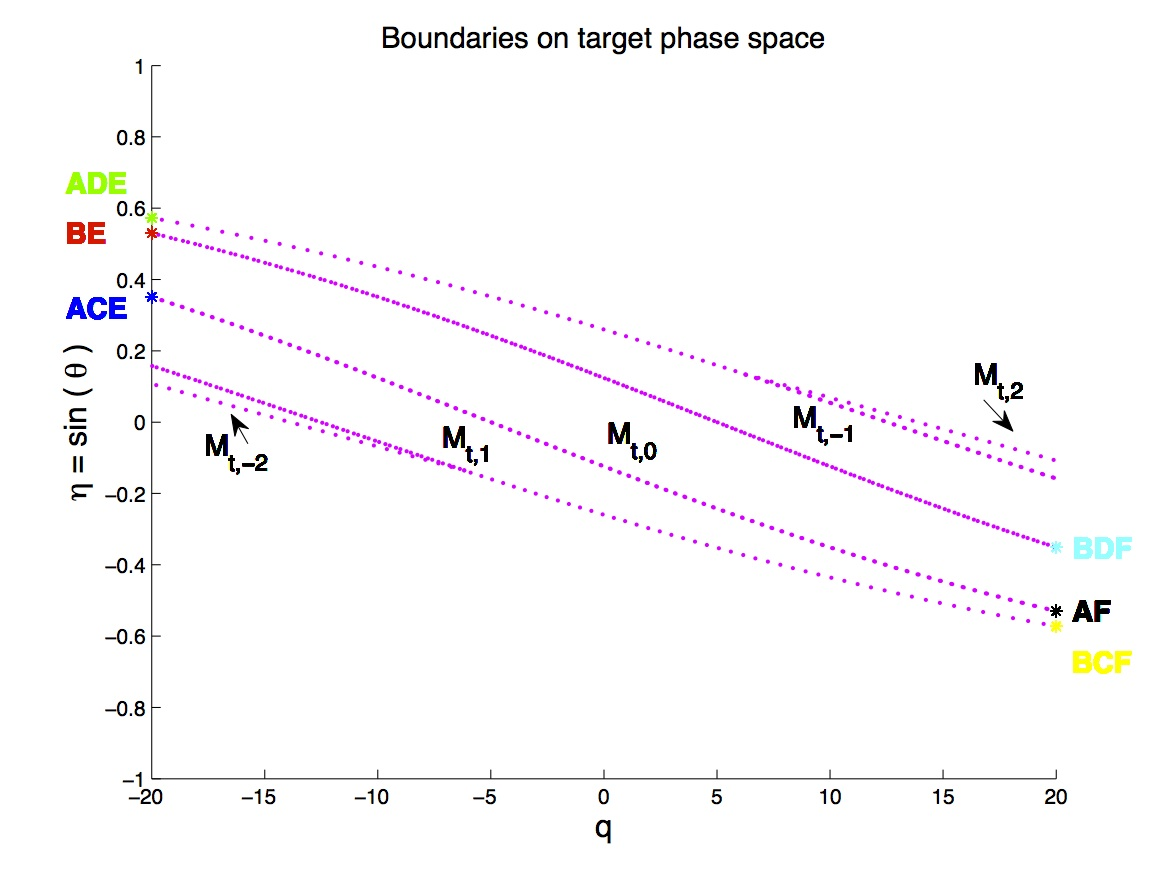
\includegraphics[scale=0.55]{boundaries_target.jpg}
\caption{Regions $M_{t,k}$ of rays that reflect $|k|$ times, for the two-faceted cup. The parameter values are: $a=5$, $b=20$ and $h=40$.}
\label{boundaries_target}
%\end{minipage} \qquad \qquad \qquad
\end{figure}
\noindent The coordinates of the rays traced in Figure $\ref{fig:raggi}$ at the target are given by:
$$ \begin{array}{cc}ADE = \big(-b, -(t_1+2\gamma)\big)),\; ACE = \big(-b, \sin(\gamma)\big),\; AF = \big(-b, -\sin(\delta)\big), \\
 BCF = \big(b, -(t_2-2\gamma)\big), BDF = \big(b, - \sin(\gamma)\big) \, \;\mbox{and} \,\; BE = \big(b, \sin(\delta)\big).\end{array} $$
 where $t_1 = \arctan(\frac(-a+b_{-1,x}{b_{-1}}))$ and $t_2 = \arctan(\frac(a-b_{-1,x}{b_{-1}}))$.


Figure $\ref{fig:boundary}$ and $\ref{boundaries_target}$ show also the symmetry of the regions $M_{\textrm{s},k}$ and $M_{\textrm{t},k}$. Finally we note that, since $k = 1$ is odd, the position of the regions $M_{\textrm{t},1}$ and $ M_{\textrm{t},-1}$ are exchanged with respect to the position of $ M_{\textrm{s},1}$ and $ M_{\textrm{s},-1}$.
